\documentclass[tikz,border=10pt]{standalone}
\usepackage[utf8]{inputenc}
\usepackage[T1]{fontenc}
\usepackage{tikz}
\usetikzlibrary{arrows.meta,fit,backgrounds}

\begin{document}
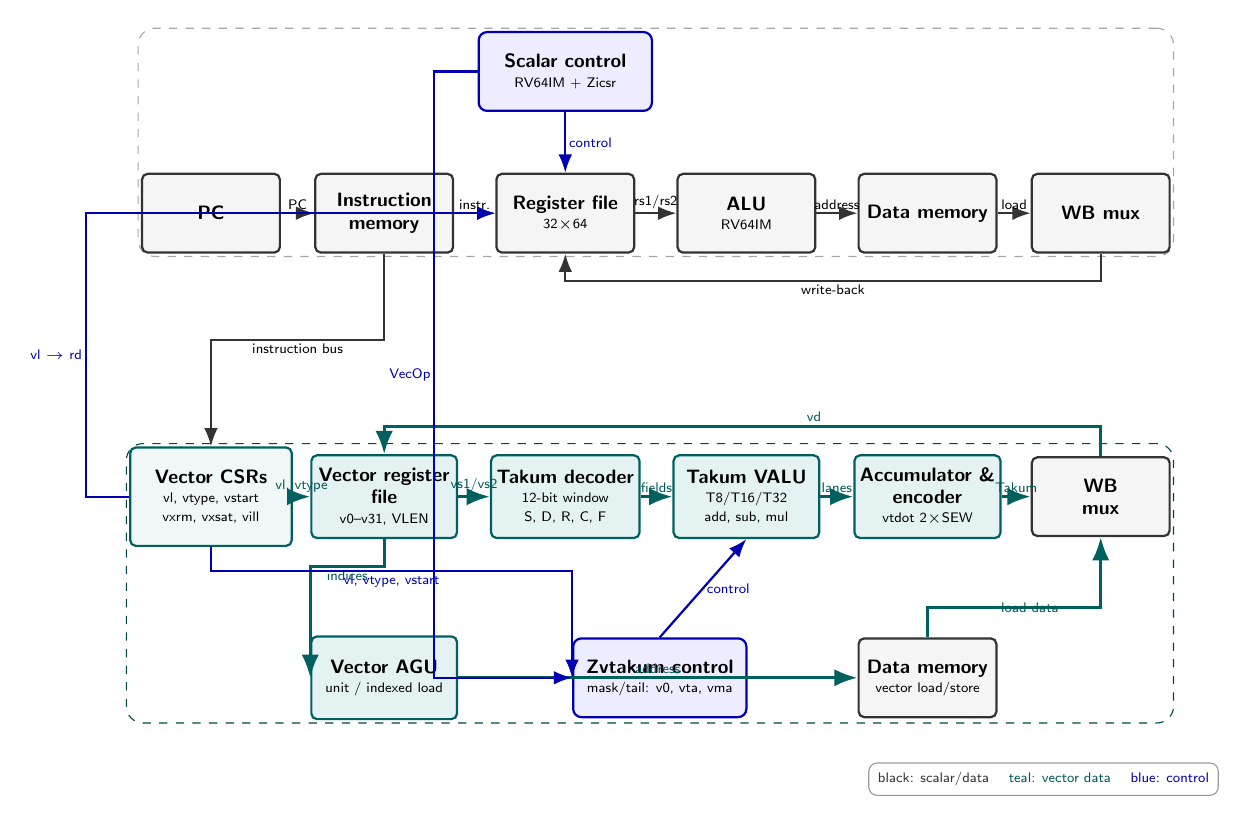
\begin{tikzpicture}[
    font=\sffamily\scriptsize,
    >=Latex,
    block/.style={draw=black!80, thick, rounded corners=2pt, fill=gray!8,
                  align=center, minimum width=1.75cm, minimum height=1.0cm, inner sep=2pt},
    vec/.style={draw=teal!75!black, thick, rounded corners=2pt, fill=teal!10,
                align=center, minimum width=1.85cm, minimum height=1.05cm, inner sep=2pt},
    ctrl/.style={draw=blue!70!black, thick, rounded corners=3pt, fill=blue!7,
                 align=center, minimum width=2.2cm, minimum height=1.0cm, inner sep=2pt},
    csr/.style={draw=teal!75!black, thick, rounded corners=2pt, fill=teal!6,
                align=center, minimum width=2.05cm, minimum height=1.25cm, inner sep=2pt},
    bus/.style={draw=black!80, thick, -{Latex}},
    vbus/.style={draw=teal!75!black, very thick, -{Latex}},
    cbus/.style={draw=blue!70!black, thick, -{Latex}},
    label/.style={font=\sffamily\tiny, inner sep=1pt},
    vlabel/.style={font=\sffamily\tiny, text=teal!70!black, inner sep=1pt},
    clabel/.style={font=\sffamily\tiny, text=blue!70!black, inner sep=1pt},
    panel/.style={draw=black!35, dashed, rounded corners=6pt, inner sep=12pt},
    vpanel/.style={draw=teal!55!black, dashed, rounded corners=6pt, inner sep=12pt}
]

% Scalar core
\node[block] (pc) at (0,3.4) {\textbf{PC}};
\node[block] (im) at (2.2,3.4) {\textbf{Instruction}\\\textbf{memory}};
\node[block] (reg) at (4.5,3.4) {\textbf{Register file}\\[-1pt]{\tiny 32$\times$64}};
\node[block] (alu) at (6.8,3.4) {\textbf{ALU}\\[-1pt]{\tiny RV64IM}};
\node[block] (dm) at (9.1,3.4) {\textbf{Data memory}};
\node[block] (wb) at (11.3,3.4) {\textbf{WB mux}};
\node[ctrl] (ctrl) at (4.5,5.2) {\textbf{Scalar control}\\[-1pt]{\tiny RV64IM + Zicsr}};

\draw[bus] (pc) -- node[label,above]{PC} (im);
\draw[bus] (im) -- node[label,above]{instr.} (reg);
\draw[bus] (reg) -- node[label,above]{rs1/rs2} (alu);
\draw[bus] (alu) -- node[label,above]{address} (dm);
\draw[bus] (dm) -- node[label,above]{load} (wb);
\draw[bus] (wb.south) -- ++(0,-0.35) -| node[label,below,pos=0.25]{write-back} (reg.south);
\draw[cbus] (ctrl.south) -- node[clabel,right]{control} (reg.north);

% Vector subsystem
\node[csr] (vcsr) at (0,-0.2) {\textbf{Vector CSRs}\\[-1pt]{\tiny vl, vtype, vstart}\\[-1pt]{\tiny vxrm, vxsat, vill}};
\node[vec] (vreg) at (2.2,-0.2) {\textbf{Vector register}\\\textbf{file}\\[-1pt]{\tiny v0--v31, VLEN}};
\node[vec] (dec) at (4.5,-0.2) {\textbf{Takum decoder}\\[-1pt]{\tiny 12-bit window}\\[-1pt]{\tiny S, D, R, C, F}};
\node[vec] (valu) at (6.8,-0.2) {\textbf{Takum VALU}\\[-1pt]{\tiny T8/T16/T32}\\[-1pt]{\tiny add, sub, mul}};
\node[vec] (acc) at (9.1,-0.2) {\textbf{Accumulator \&}\\\textbf{encoder}\\[-1pt]{\tiny vtdot 2$\times$SEW}};
\node[block] (muxv) at (11.3,-0.2) {\textbf{WB}\\\textbf{mux}};
\node[vec] (agu) at (2.2,-2.5) {\textbf{Vector AGU}\\[-1pt]{\tiny unit / indexed load}};
\node[ctrl] (zctl) at (5.7,-2.5) {\textbf{Zvtakum control}\\[-1pt]{\tiny mask/tail: v0, vta, vma}};
\node[block] (vmem) at (9.1,-2.5) {\textbf{Data memory}\\[-1pt]{\tiny vector load/store}};

\draw[vbus] (vcsr) -- node[vlabel,above]{vl, vtype} (vreg);
\draw[vbus] (vreg) -- node[vlabel,above]{vs1/vs2} (dec);
\draw[vbus] (dec) -- node[vlabel,above]{fields} (valu);
\draw[vbus] (valu) -- node[vlabel,above]{lanes} (acc);
\draw[vbus] (acc) -- node[vlabel,above]{Takum} (muxv);
\draw[vbus] (muxv.north) -- ++(0,0.38) -| node[vlabel,above,pos=0.2]{vd} (vreg.north);
\draw[vbus] (vreg.south) -- ++(0,-0.35) -| node[vlabel,below,pos=0.25]{indices} (agu.west);
\draw[vbus] (agu) -- node[vlabel,above]{address} (vmem);
\draw[vbus] (vmem.north) -- ++(0,0.38) -| node[vlabel,right,pos=0.2]{load data} (muxv.south);
\draw[cbus] (zctl.north) -- node[clabel,right]{control} (valu.south);
\draw[cbus] (vcsr.south) -- ++(0,-0.3) -| node[clabel,below,pos=0.25]{vl, vtype, vstart} (zctl.west);

% Instruction bus and scalar/vector interaction
\draw[bus] (im.south) -- ++(0,-1.1) -| node[label,below,pos=0.25]{instruction bus} (vcsr.north);
\draw[cbus] (ctrl.west) -- ++(-0.55,0) |- node[clabel,left,pos=0.25]{VecOp} (zctl.west);
\draw[cbus] (vcsr.west) -- ++(-0.55,0) |- node[clabel,left,pos=0.25]{vl $\rightarrow$ rd} (reg.west);

% Panels
\begin{scope}[on background layer]
    \node[panel, fit=(pc) (im) (reg) (alu) (dm) (wb) (ctrl),
          label={[anchor=south west,font=\sffamily\bfseries\scriptsize]above left:RV64IM scalar core (functional)}] {};
    \node[vpanel, fit=(vcsr) (vreg) (dec) (valu) (acc) (muxv) (agu) (zctl) (vmem),
          label={[anchor=north west,font=\sffamily\bfseries\scriptsize,text=teal!70!black]below left:Zvtakum vector subsystem (T8/T16/T32)}] {};
\end{scope}

\node[draw=black!40, rounded corners=3pt, fill=white, font=\sffamily\tiny,
      anchor=south east] at (12.8,-4.0) {%
    \textcolor{black!80}{black: scalar/data} \quad
    \textcolor{teal!70!black}{teal: vector data} \quad
    \textcolor{blue!70!black}{blue: control}%
};

\end{tikzpicture}
\end{document}
